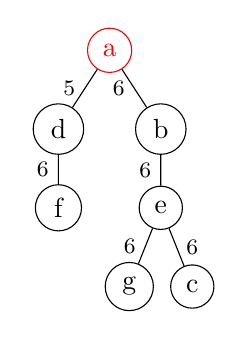
\begin{tikzpicture}[
    level distance = 1cm,
    level 1/.style = {sibling distance=1.3cm},
    level 2/.style = {sibling distance=1.0cm},
    level 3/.style = {sibling distance=0.8cm},
    every node/.style = {circle,draw},
    lbl/.style = {rectangle, draw=none, #1,% position
    font=\footnotesize}
    ]
    %
    \node (Root) [red] {a}
        child {node {d}
            child {node {f}
                edge from parent node[lbl=left] {$6$}
            }
            edge from parent node[lbl=left] {$5$}
        }
        child { node {b}
            child { node {e} 
                child{ 
                    node {g} 
                    edge from parent node[lbl=left] {$6$}
                }
                child{ 
                    node {c}
                    edge from parent node[lbl=right] {$6$}
                }
                edge from parent node[lbl=left] {$6$}
            }
            edge from parent node[lbl=left] {$6$}
        };
\end{tikzpicture}

